\documentclass{standalone}
\usepackage{tikz}
\usetikzlibrary{patterns, positioning}


\begin{document}
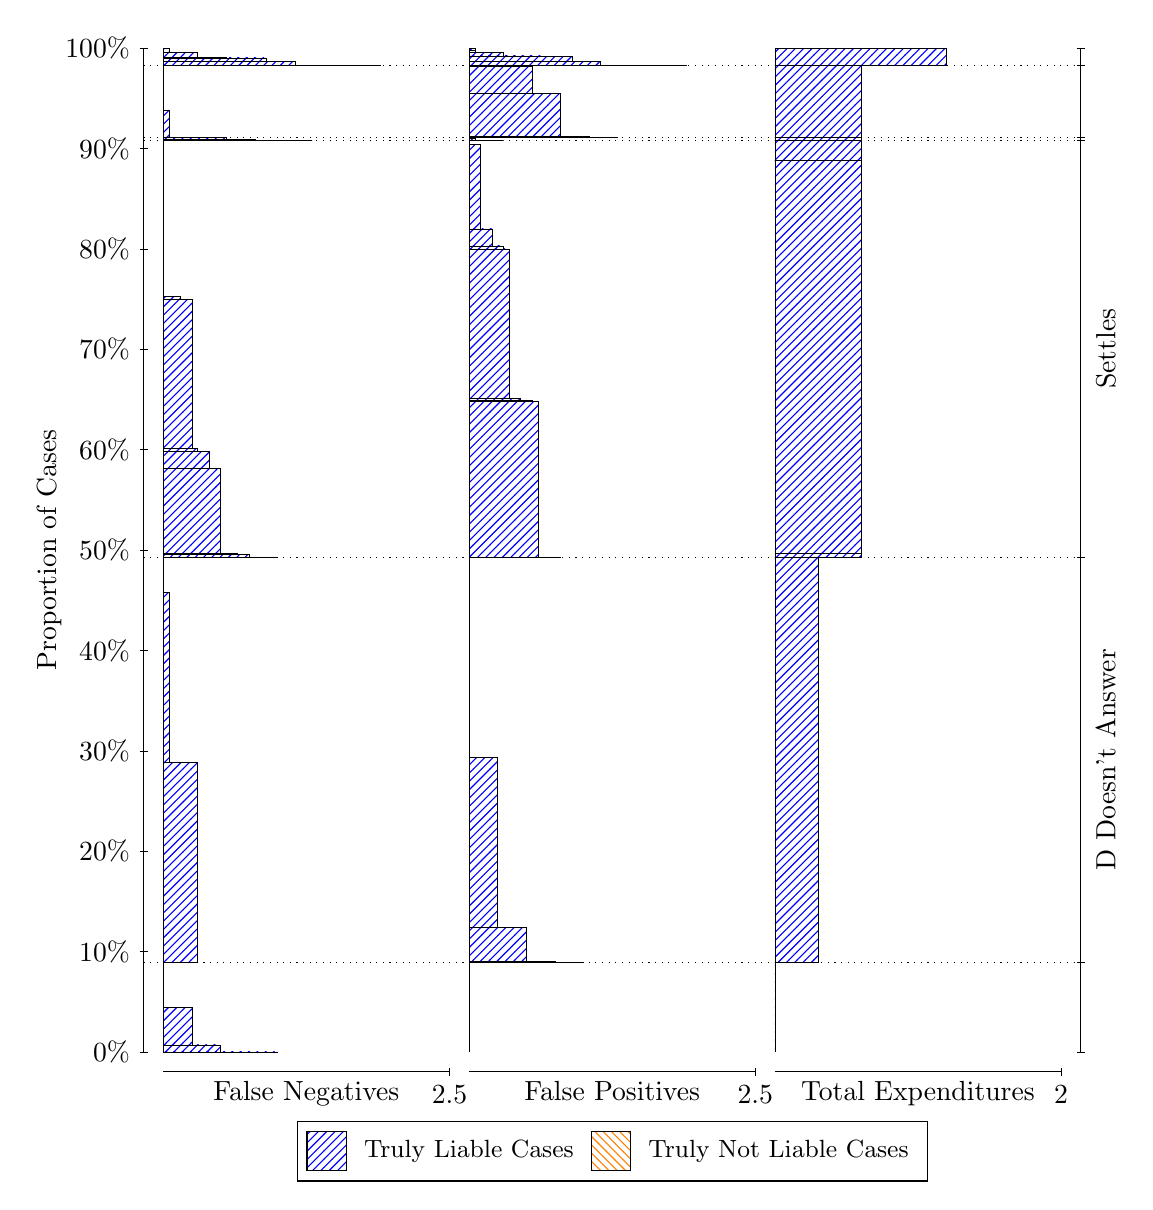
\begin{tikzpicture}
\draw[black, very thin] (1.5,1.75) -- (1.5,14.5);
\node[rotate=90, text=black, anchor=center] at (0.3, 8.125) {Proportion of Cases};
\draw[black, very thin] (1.45,1.75) -- (1.55,1.75);
\node[text=black, anchor=east] at (1.45, 1.75) {0\%};
\draw[black, very thin] (1.45,3.025) -- (1.55,3.025);
\node[text=black, anchor=east] at (1.45, 3.025) {10\%};
\draw[black, very thin] (1.45,4.3) -- (1.55,4.3);
\node[text=black, anchor=east] at (1.45, 4.3) {20\%};
\draw[black, very thin] (1.45,5.575) -- (1.55,5.575);
\node[text=black, anchor=east] at (1.45, 5.575) {30\%};
\draw[black, very thin] (1.45,6.85) -- (1.55,6.85);
\node[text=black, anchor=east] at (1.45, 6.85) {40\%};
\draw[black, very thin] (1.45,8.125) -- (1.55,8.125);
\node[text=black, anchor=east] at (1.45, 8.125) {50\%};
\draw[black, very thin] (1.45,9.4) -- (1.55,9.4);
\node[text=black, anchor=east] at (1.45, 9.4) {60\%};
\draw[black, very thin] (1.45,10.675) -- (1.55,10.675);
\node[text=black, anchor=east] at (1.45, 10.675) {70\%};
\draw[black, very thin] (1.45,11.95) -- (1.55,11.95);
\node[text=black, anchor=east] at (1.45, 11.95) {80\%};
\draw[black, very thin] (1.45,13.225) -- (1.55,13.225);
\node[text=black, anchor=east] at (1.45, 13.225) {90\%};
\draw[black, very thin] (1.45,14.5) -- (1.55,14.5);
\node[text=black, anchor=east] at (1.45, 14.5) {100\%};

\draw[black, very thin] (13.4,1.75) -- (13.4,14.5);
\draw[black, very thin] (13.35,1.75) -- (13.45,1.75);
\node[anchor=west] at (13.35, 1.75) {};
\draw[black, very thin] (13.35,2.8831) -- (13.45,2.8831);
\node[anchor=west] at (13.35, 2.8831) {};
\draw[black, very thin] (13.35,8.034) -- (13.45,8.034);
\node[anchor=west] at (13.35, 8.034) {};
\draw[black, very thin] (13.35,13.329) -- (13.45,13.329);
\node[anchor=west] at (13.35, 13.329) {};
\draw[black, very thin] (13.35,13.365) -- (13.45,13.365);
\node[anchor=west] at (13.35, 13.365) {};
\draw[black, very thin] (13.35,14.276) -- (13.45,14.276);
\node[anchor=west] at (13.35, 14.276) {};
\draw[black, very thin] (13.35,14.5) -- (13.45,14.5);
\node[anchor=west] at (13.35, 14.5) {};

\draw[black, very thin, pattern color=blue, pattern=north east lines] (1.75,1.75) rectangle (3.2033,1.75);
\draw[black, very thin, pattern color=blue, pattern=north east lines] (1.75,1.75) rectangle (2.84,1.7508);
\draw[black, very thin, pattern color=blue, pattern=north east lines] (1.75,1.7508) rectangle (2.4767,1.8407);
\draw[black, very thin, pattern color=blue, pattern=north east lines] (1.75,1.8407) rectangle (2.1133,2.3173);
\draw[black, very thin, pattern color=orange, pattern=north west lines] (1.75,2.3173) rectangle (1.75,2.3173);
\draw[black, very thin, pattern color=blue, pattern=north east lines] (1.75,2.3173) rectangle (1.75,2.8831);
\draw[black, very thin, pattern color=blue, pattern=north east lines] (1.75,2.8831) rectangle (2.186,5.429);
\draw[black, very thin, pattern color=blue, pattern=north east lines] (1.75,5.429) rectangle (1.8227,7.5839);
\draw[black, very thin, pattern color=orange, pattern=north west lines] (1.75,7.5839) rectangle (1.75,7.5839);
\draw[black, very thin, pattern color=blue, pattern=north east lines] (1.75,7.5839) rectangle (1.75,8.034);
\draw[black, very thin, pattern color=blue, pattern=north east lines] (1.75,8.034) rectangle (3.2033,8.034);
\draw[black, very thin, pattern color=blue, pattern=north east lines] (1.75,8.034) rectangle (3.058,8.034);
\draw[black, very thin, pattern color=blue, pattern=north east lines] (1.75,8.034) rectangle (2.9127,8.034);
\draw[black, very thin, pattern color=blue, pattern=north east lines] (1.75,8.034) rectangle (2.84,8.0693);
\draw[black, very thin, pattern color=blue, pattern=north east lines] (1.75,8.0693) rectangle (2.6947,8.0797);
\draw[black, very thin, pattern color=blue, pattern=north east lines] (1.75,8.0797) rectangle (2.5493,8.0815);
\draw[black, very thin, pattern color=blue, pattern=north east lines] (1.75,8.0815) rectangle (2.4767,9.1596);
\draw[black, very thin, pattern color=blue, pattern=north east lines] (1.75,9.1596) rectangle (2.3313,9.376);
\draw[black, very thin, pattern color=blue, pattern=north east lines] (1.75,9.376) rectangle (2.186,9.4123);
\draw[black, very thin, pattern color=blue, pattern=north east lines] (1.75,9.4123) rectangle (2.1133,11.308);
\draw[black, very thin, pattern color=blue, pattern=north east lines] (1.75,11.308) rectangle (1.968,11.341);
\draw[black, very thin, pattern color=blue, pattern=north east lines] (1.75,11.341) rectangle (1.8227,11.346);
\draw[black, very thin, pattern color=orange, pattern=north west lines] (1.75,11.346) rectangle (1.75,11.346);
\draw[black, very thin, pattern color=blue, pattern=north east lines] (1.75,11.346) rectangle (1.75,13.329);
\draw[black, very thin, pattern color=blue, pattern=north east lines] (1.75,13.329) rectangle (3.6393,13.329);
\draw[black, very thin, pattern color=blue, pattern=north east lines] (1.75,13.329) rectangle (3.276,13.329);
\draw[black, very thin, pattern color=blue, pattern=north east lines] (1.75,13.329) rectangle (2.9127,13.341);
\draw[black, very thin, pattern color=blue, pattern=north east lines] (1.75,13.341) rectangle (2.5493,13.364);
\draw[black, very thin, pattern color=blue, pattern=north east lines] (1.75,13.364) rectangle (2.186,13.365);
\draw[black, very thin, pattern color=orange, pattern=north west lines] (1.75,13.365) rectangle (1.75,13.365);
\draw[black, very thin, pattern color=blue, pattern=north east lines] (1.75,13.365) rectangle (2.186,13.369);
\draw[black, very thin, pattern color=blue, pattern=north east lines] (1.75,13.369) rectangle (1.8227,13.713);
\draw[black, very thin, pattern color=orange, pattern=north west lines] (1.75,13.713) rectangle (1.75,13.713);
\draw[black, very thin, pattern color=blue, pattern=north east lines] (1.75,13.713) rectangle (1.75,14.276);
\draw[black, very thin, pattern color=blue, pattern=north east lines] (1.75,14.276) rectangle (4.5113,14.276);
\draw[black, very thin, pattern color=blue, pattern=north east lines] (1.75,14.276) rectangle (4.148,14.276);
\draw[black, very thin, pattern color=blue, pattern=north east lines] (1.75,14.276) rectangle (3.7847,14.279);
\draw[black, very thin, pattern color=blue, pattern=north east lines] (1.75,14.279) rectangle (3.4213,14.329);
\draw[black, very thin, pattern color=blue, pattern=north east lines] (1.75,14.329) rectangle (3.276,14.329);
\draw[black, very thin, pattern color=blue, pattern=north east lines] (1.75,14.329) rectangle (3.058,14.376);
\draw[black, very thin, pattern color=blue, pattern=north east lines] (1.75,14.376) rectangle (2.9127,14.376);
\draw[black, very thin, pattern color=blue, pattern=north east lines] (1.75,14.376) rectangle (2.6947,14.376);
\draw[black, very thin, pattern color=blue, pattern=north east lines] (1.75,14.376) rectangle (2.5493,14.377);
\draw[black, very thin, pattern color=blue, pattern=north east lines] (1.75,14.377) rectangle (2.3313,14.377);
\draw[black, very thin, pattern color=blue, pattern=north east lines] (1.75,14.377) rectangle (2.186,14.377);
\draw[black, very thin, pattern color=blue, pattern=north east lines] (1.75,14.377) rectangle (2.186,14.443);
\draw[black, very thin, pattern color=blue, pattern=north east lines] (1.75,14.443) rectangle (1.8227,14.444);
\draw[black, very thin, pattern color=blue, pattern=north east lines] (1.75,14.444) rectangle (1.8227,14.495);
\draw[black, very thin, pattern color=orange, pattern=north west lines] (1.75,14.495) rectangle (1.75,14.495);
\draw[black, very thin, pattern color=blue, pattern=north east lines] (1.75,14.495) rectangle (1.75,14.5);
\draw[black, very thin, pattern color=orange, pattern=north west lines] (5.6333,1.75) rectangle (5.6333,1.75);
\draw[black, very thin, pattern color=blue, pattern=north east lines] (5.6333,1.75) rectangle (5.6333,2.8831);
\draw[black, very thin, pattern color=orange, pattern=north west lines] (5.6333,2.8831) rectangle (7.0867,2.8831);
\draw[black, very thin, pattern color=blue, pattern=north east lines] (5.6333,2.8831) rectangle (7.0867,2.8832);
\draw[black, very thin, pattern color=blue, pattern=north east lines] (5.6333,2.8832) rectangle (6.7233,2.8966);
\draw[black, very thin, pattern color=blue, pattern=north east lines] (5.6333,2.8966) rectangle (6.36,3.3332);
\draw[black, very thin, pattern color=blue, pattern=north east lines] (5.6333,3.3332) rectangle (5.9967,5.4881);
\draw[black, very thin, pattern color=blue, pattern=north east lines] (5.6333,5.4881) rectangle (5.6333,8.034);
\draw[black, very thin, pattern color=orange, pattern=north west lines] (5.6333,8.034) rectangle (6.796,8.034);
\draw[black, very thin, pattern color=blue, pattern=north east lines] (5.6333,8.034) rectangle (6.796,8.034);
\draw[black, very thin, pattern color=orange, pattern=north west lines] (5.6333,8.034) rectangle (6.6507,8.034);
\draw[black, very thin, pattern color=blue, pattern=north east lines] (5.6333,8.034) rectangle (6.6507,8.0341);
\draw[black, very thin, pattern color=orange, pattern=north west lines] (5.6333,8.0341) rectangle (6.5053,8.0341);
\draw[black, very thin, pattern color=blue, pattern=north east lines] (5.6333,8.0341) rectangle (6.5053,10.016);
\draw[black, very thin, pattern color=blue, pattern=north east lines] (5.6333,10.016) rectangle (6.4327,10.022);
\draw[black, very thin, pattern color=blue, pattern=north east lines] (5.6333,10.022) rectangle (6.2873,10.054);
\draw[black, very thin, pattern color=blue, pattern=north east lines] (5.6333,10.054) rectangle (6.142,11.95);
\draw[black, very thin, pattern color=blue, pattern=north east lines] (5.6333,11.95) rectangle (6.0693,11.987);
\draw[black, very thin, pattern color=blue, pattern=north east lines] (5.6333,11.987) rectangle (5.924,12.203);
\draw[black, very thin, pattern color=blue, pattern=north east lines] (5.6333,12.203) rectangle (5.7787,13.281);
\draw[black, very thin, pattern color=blue, pattern=north east lines] (5.6333,13.281) rectangle (5.706,13.283);
\draw[black, very thin, pattern color=blue, pattern=north east lines] (5.6333,13.283) rectangle (5.6333,13.329);
\draw[black, very thin, pattern color=orange, pattern=north west lines] (5.6333,13.329) rectangle (6.0693,13.329);
\draw[black, very thin, pattern color=blue, pattern=north east lines] (5.6333,13.329) rectangle (6.0693,13.329);
\draw[black, very thin, pattern color=blue, pattern=north east lines] (5.6333,13.329) rectangle (5.706,13.352);
\draw[black, very thin, pattern color=blue, pattern=north east lines] (5.6333,13.352) rectangle (5.6333,13.365);
\draw[black, very thin, pattern color=orange, pattern=north west lines] (5.6333,13.365) rectangle (7.5227,13.365);
\draw[black, very thin, pattern color=blue, pattern=north east lines] (5.6333,13.365) rectangle (7.5227,13.365);
\draw[black, very thin, pattern color=blue, pattern=north east lines] (5.6333,13.365) rectangle (7.1593,13.38);
\draw[black, very thin, pattern color=blue, pattern=north east lines] (5.6333,13.38) rectangle (6.796,13.928);
\draw[black, very thin, pattern color=blue, pattern=north east lines] (5.6333,13.928) rectangle (6.4327,14.272);
\draw[black, very thin, pattern color=blue, pattern=north east lines] (5.6333,14.272) rectangle (6.0693,14.276);
\draw[black, very thin, pattern color=orange, pattern=north west lines] (5.6333,14.276) rectangle (8.3947,14.276);
\draw[black, very thin, pattern color=blue, pattern=north east lines] (5.6333,14.276) rectangle (8.3947,14.276);
\draw[black, very thin, pattern color=orange, pattern=north west lines] (5.6333,14.276) rectangle (8.0313,14.276);
\draw[black, very thin, pattern color=blue, pattern=north east lines] (5.6333,14.276) rectangle (8.0313,14.276);
\draw[black, very thin, pattern color=orange, pattern=north west lines] (5.6333,14.276) rectangle (7.668,14.276);
\draw[black, very thin, pattern color=blue, pattern=north east lines] (5.6333,14.276) rectangle (7.668,14.281);
\draw[black, very thin, pattern color=orange, pattern=north west lines] (5.6333,14.281) rectangle (7.3047,14.281);
\draw[black, very thin, pattern color=blue, pattern=north east lines] (5.6333,14.281) rectangle (7.3047,14.332);
\draw[black, very thin, pattern color=blue, pattern=north east lines] (5.6333,14.332) rectangle (6.9413,14.398);
\draw[black, very thin, pattern color=orange, pattern=north west lines] (5.6333,14.398) rectangle (6.796,14.398);
\draw[black, very thin, pattern color=blue, pattern=north east lines] (5.6333,14.398) rectangle (6.796,14.398);
\draw[black, very thin, pattern color=blue, pattern=north east lines] (5.6333,14.398) rectangle (6.578,14.4);
\draw[black, very thin, pattern color=orange, pattern=north west lines] (5.6333,14.4) rectangle (6.4327,14.4);
\draw[black, very thin, pattern color=blue, pattern=north east lines] (5.6333,14.4) rectangle (6.4327,14.4);
\draw[black, very thin, pattern color=blue, pattern=north east lines] (5.6333,14.4) rectangle (6.2147,14.4);
\draw[black, very thin, pattern color=blue, pattern=north east lines] (5.6333,14.4) rectangle (6.0693,14.446);
\draw[black, very thin, pattern color=orange, pattern=north west lines] (5.6333,14.446) rectangle (6.0693,14.446);
\draw[black, very thin, pattern color=blue, pattern=north east lines] (5.6333,14.446) rectangle (6.0693,14.447);
\draw[black, very thin, pattern color=blue, pattern=north east lines] (5.6333,14.447) rectangle (5.8513,14.447);
\draw[black, very thin, pattern color=blue, pattern=north east lines] (5.6333,14.447) rectangle (5.706,14.476);
\draw[black, very thin, pattern color=blue, pattern=north east lines] (5.6333,14.476) rectangle (5.706,14.497);
\draw[black, very thin, pattern color=blue, pattern=north east lines] (5.6333,14.497) rectangle (5.6333,14.5);
\draw[black, very thin, pattern color=orange, pattern=north west lines] (9.5167,1.75) rectangle (9.5167,1.75);
\draw[black, very thin, pattern color=blue, pattern=north east lines] (9.5167,1.75) rectangle (9.5167,2.8831);
\draw[black, very thin, pattern color=orange, pattern=north west lines] (9.5167,2.8831) rectangle (10.062,2.8831);
\draw[black, very thin, pattern color=blue, pattern=north east lines] (9.5167,2.8831) rectangle (10.062,8.034);
\draw[black, very thin, pattern color=orange, pattern=north west lines] (9.5167,8.034) rectangle (10.607,8.034);
\draw[black, very thin, pattern color=blue, pattern=north east lines] (9.5167,8.034) rectangle (10.607,8.0775);
\draw[black, very thin, pattern color=orange, pattern=north west lines] (9.5167,8.0775) rectangle (10.607,8.0775);
\draw[black, very thin, pattern color=blue, pattern=north east lines] (9.5167,8.0775) rectangle (10.607,13.069);
\draw[black, very thin, pattern color=orange, pattern=north west lines] (9.5167,13.069) rectangle (10.607,13.069);
\draw[black, very thin, pattern color=blue, pattern=north east lines] (9.5167,13.069) rectangle (10.607,13.329);
\draw[black, very thin, pattern color=orange, pattern=north west lines] (9.5167,13.329) rectangle (10.607,13.329);
\draw[black, very thin, pattern color=blue, pattern=north east lines] (9.5167,13.329) rectangle (10.607,13.365);
\draw[black, very thin, pattern color=orange, pattern=north west lines] (9.5167,13.365) rectangle (10.607,13.365);
\draw[black, very thin, pattern color=blue, pattern=north east lines] (9.5167,13.365) rectangle (10.607,14.276);
\draw[black, very thin, pattern color=orange, pattern=north west lines] (9.5167,14.276) rectangle (11.697,14.276);
\draw[black, very thin, pattern color=blue, pattern=north east lines] (9.5167,14.276) rectangle (11.697,14.5);
\draw[black, dotted] (1.5,2.8831) -- (13.4,2.8831);
\draw[black, dotted] (1.5,8.034) -- (13.4,8.034);
\draw[black, dotted] (1.5,13.329) -- (13.4,13.329);
\draw[black, dotted] (1.5,13.365) -- (13.4,13.365);
\draw[black, dotted] (1.5,14.276) -- (13.4,14.276);
\draw[black, very thin] (1.75,1.5) -- (5.3833,1.5);
\node[text=black, anchor=north] at (3.5667, 1.5) {False Negatives};
\draw[black, very thin] (5.3833,1.45) -- (5.3833,1.55);
\node[text=black, anchor=north] at (5.3833, 1.45) {2.5};

\draw[black, very thin] (5.6333,1.5) -- (9.2667,1.5);
\node[text=black, anchor=north] at (7.45, 1.5) {False Positives};
\draw[black, very thin] (9.2667,1.45) -- (9.2667,1.55);
\node[text=black, anchor=north] at (9.2667, 1.45) {2.5};

\draw[black, very thin] (9.5167,1.5) -- (13.15,1.5);
\node[text=black, anchor=north] at (11.333, 1.5) {Total Expenditures};
\draw[black, very thin] (13.15,1.45) -- (13.15,1.55);
\node[text=black, anchor=north] at (13.15, 1.45) {2};


\node[text=black, centered, rotate=90] at (13.72, 5.4585) {D Doesn't Answer};
\node[text=black, centered, rotate=90] at (13.72, 10.681) {Settles};




\draw (7.449999999999999,1.5) node[draw=none] (baseCoordinate) {};
\begin{scope}[align=center]
        \matrix[scale=0.5, draw=black, below=0.5cm of baseCoordinate, nodes={draw}, column sep=0.1cm]{
            \node[rectangle, draw, minimum width=0.5cm, minimum height=0.5cm, pattern color=blue, pattern=north east lines] {}; &
            \node[draw=none, font=\small, text=black] (B) {Truly Liable Cases}; &
            \node[rectangle, draw, minimum width=0.5cm, minimum height=0.5cm, pattern color=orange, pattern=north west lines] {}; &
            \node[draw=none, font=\small, text=black] (B) {Truly Not Liable Cases}; \\
            };
\end{scope}

\end{tikzpicture}
\end{document}